\documentclass{beamer}


\usepackage[utf8]{inputenc}   % Підтримка UTF-8
\usepackage[ukrainian]{babel} % Підтримка української мови
\usepackage[ukrainian=nohyphenation]{hyphsubst}
\usepackage[T2A]{fontenc}      % Кодова таблиця для кирилиці

\usepackage{booktabs}
\usepackage{amsmath, amsfonts} % Для математики, якщо потрібно
\usepackage{hyperref}          % Для створення посилань
\usepackage{listings}          % Пакет для вставки коду
\usepackage{graphicx}
\usepackage{csvsimple}
\usepackage{parskip}
\usepackage{csquotes}
\usepackage{xcolor}
\usepackage{multicol} % Для багатостовпчикового тексту

\usepackage{tabularray}
\usepackage{float}
\usepackage{codehigh}
\usepackage[normalem]{ulem}

\UseTblrLibrary{booktabs}
\UseTblrLibrary{siunitx}
\newcommand{\tinytableTabularrayUnderline}[1]{\underline{#1}}
\newcommand{\tinytableTabularrayStrikeout}[1]{\sout{#1}}
\NewTableCommand{\tinytableDefineColor}[3]{\definecolor{#1}{#2}{#3}}

\usetheme{Madrid}

% Прибираєм навігацію з кожного слайду
\beamertemplatenavigationsymbolsempty

\title{Лабораторна робота №4}
\subtitle{Непараметрична регресiя. Аналіз головних компонент }
\subtitle{Команда №9}

% [], щоб прибрати імена з кожного слайду
\author[]{
  Баранівська В.О.,
  Корсун Є. В.,
  Хмарук О. Ю.,
  Літковський А.С.,
  Кудін Н. А.
}
\date{2025}

\begin{document}

\frame{\titlepage}

\graphicspath{{../../../}} % Ensure this path is correct or remove it if not needed

%Короткий підсумок ЛР 1-2 (якщо є свіжі погляди, можна ще зменшити/додати/змінити)

\begin{frame}
  \section{Набір даних}

  \frametitle{Зміст}
  \tableofcontents[currentsection]
\end{frame}

\begin{frame}
  \frametitle{Набір даних}

  Було вирішено дослідити якість повітря Тайваню. Уряд провінції намагається
  контролювати та покращувати якість повітря. Тому 17 грудня 2017 року була введена
  реформа \textit{Air Pollution Control Action Plan}.

  \begin{center}

  \end{center}
\end{frame}

\begin{frame}
  \frametitle{Висновки EDA}
  \begin{itemize}
    \item Загальний рівень AQI по регіонам зменшується, тобто показники покращуються після початку реформи.
    Більш явні зміни очікувано помітні через декілька років після реформи.
    \item Якість повітря змінюється нерівномірно у містах.
  \end{itemize}
\end{frame}

\begin{frame}
  \frametitle{Питання для дослідження}
  Як реформа покращення якості повітря вплинула на якість повітря,
  враховуючи можливі нелінійні залежності та взаємодії між факторами?
\end{frame}

% Описати, чи використовується той самий агрегований (по днях, медіани) датасет, що і в ЛР3.
% Зазначити, чи потрібна додаткова обробка (наприклад, робота з викидами, якщо вони сильно впливають на непараметричні оцінки).
\begin{frame}
  \frametitle{Підготовка даних для непараметричної регресії}
  \begin{itemize}
    \item \textbf{Дані:} агреговані по днях з використанням медіанних значень для зменшення впливу викидів та шуму в погодинних даних.
    \item \textbf{Цільова змінна:} AQI (Air Quality Index).
    \item \textbf{Основні регресори для непараметричного аналізу:}
        \begin{itemize}
            \item \texttt{reform\_days}: кількість днів з моменту початку реформи (для оцінки впливу реформи).
            \item \texttt{windspeed}: швидкість вітру (для дослідження нелінійного впливу погодних умов).
            \item \texttt{july\_days}: кількість днів з початку липня (для врахування сезонності).
        \end{itemize}
    \item \textbf{Розбиття датасету:} на тренувальний та тестовий (80\%/20\%) для оцінки якості моделей.
  \end{itemize}
\end{frame}

\begin{frame}
  \section{Ядрова регресія (непараметрична)}

  \frametitle{Зміст}
  \tableofcontents[currentsection]
\end{frame}

\begin{frame}
  \frametitle{Ядрова регресія}

  \begin{center}
    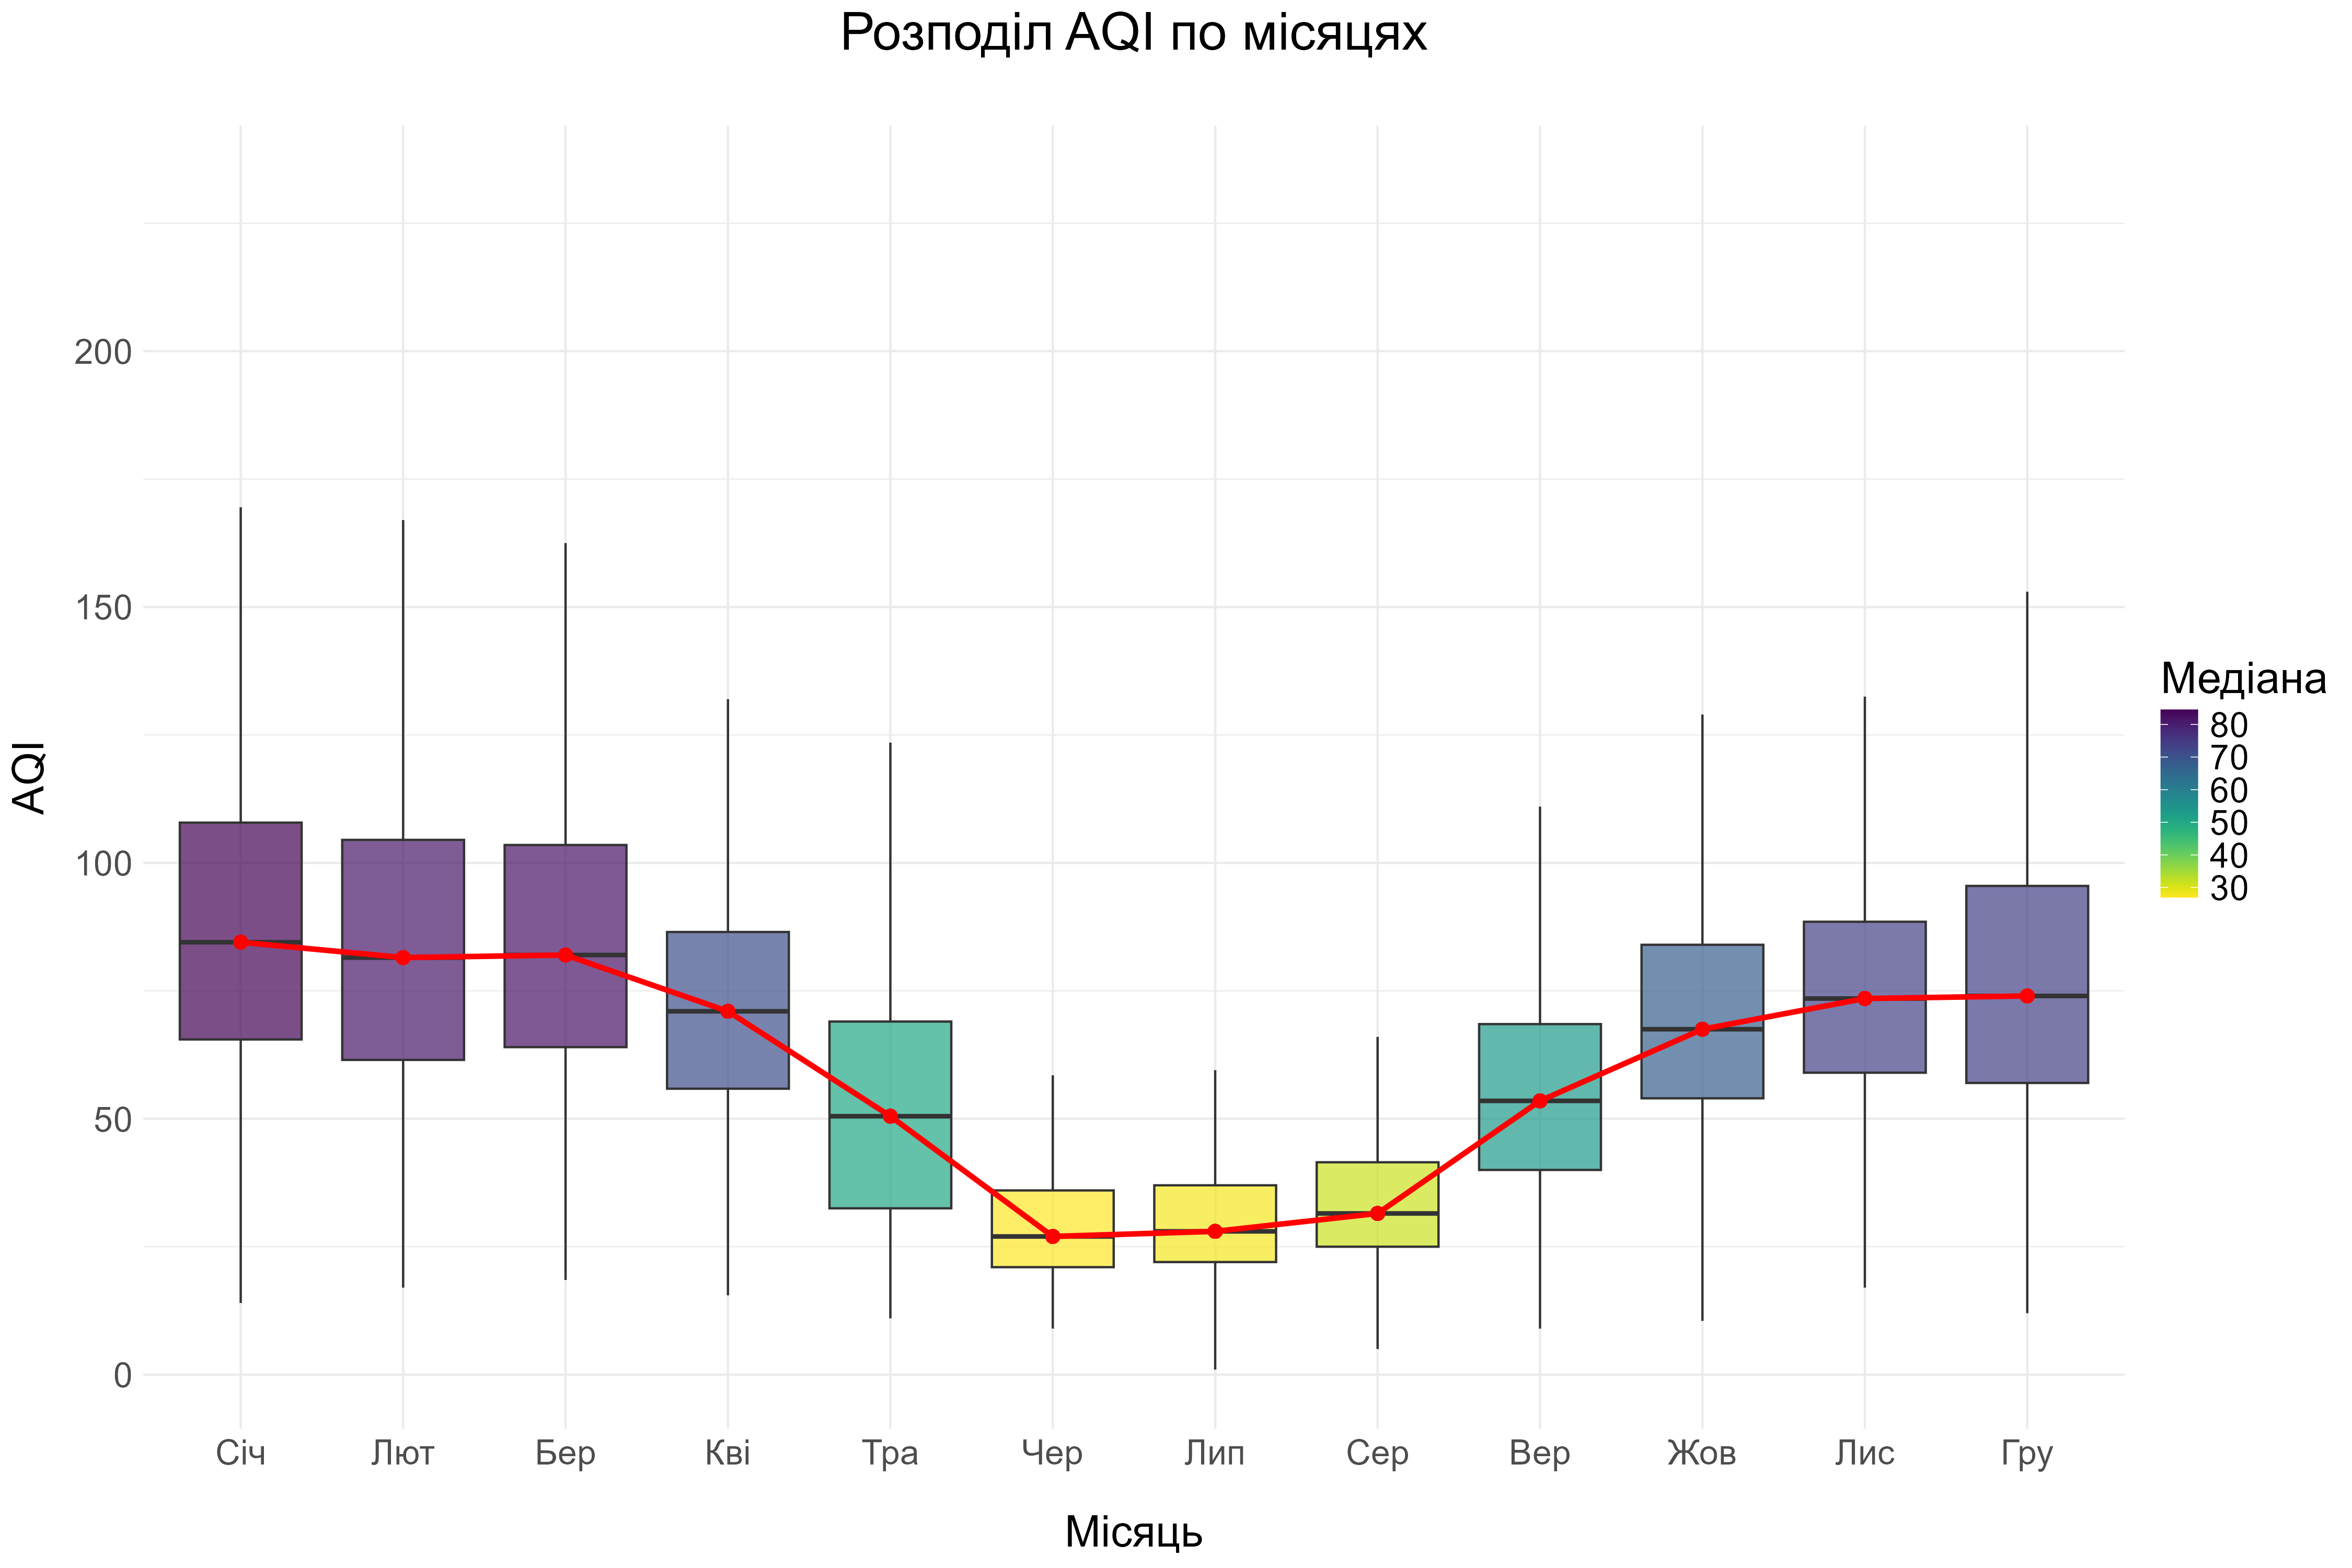
\includegraphics[height=2.8in]{plots/lab4/kernal/seasonal_change_median_line.png}
  \end{center}

  %Ядрова регресія — це непараметричний метод оцінки умовної математичної сподіваності залежної змінної $Y$ при заданому значенні незалежної змінної $X=x$.
  %\begin{itemize}
  %  \item \textbf{Оцінка Надарая-Вотсона (Nadaraya-Watson Estimator):}
  %  Найбільш поширена форма ядрової регресії. Оцінка функції регресії $m(x) = E[Y|X=x]$ в точці $x$ задається як:
  %  $$ \hat{m}_h(x) = \frac{\sum_{i=1}^{n} K_h(x - X_i) Y_i}{\sum_{i=1}^{n} K_h(x - X_i)} $$
  %  де:
  %  \begin{itemize}
  %      \item $n$ – кількість спостережень.
  %      \item $Y_i$ – значення залежної змінної для $i$-го спостереження.
  %      \item $X_i$ – значення незалежної змінної для $i$-го спостереження.
  %      \item $K_h(u) = \frac{1}{h}K(\frac{u}{h})$ – масштабоване ядро.
  %      \item $K(\cdot)$ – ядрова функція (kernel function).
  %      \item $h$ – параметр згладжування (bandwidth або ширина вікна).
  %  \end{itemize}
  %\end{itemize}
\end{frame}

\begin{frame}
  \frametitle{Ядрова регресія}
  
  \begin{center}
    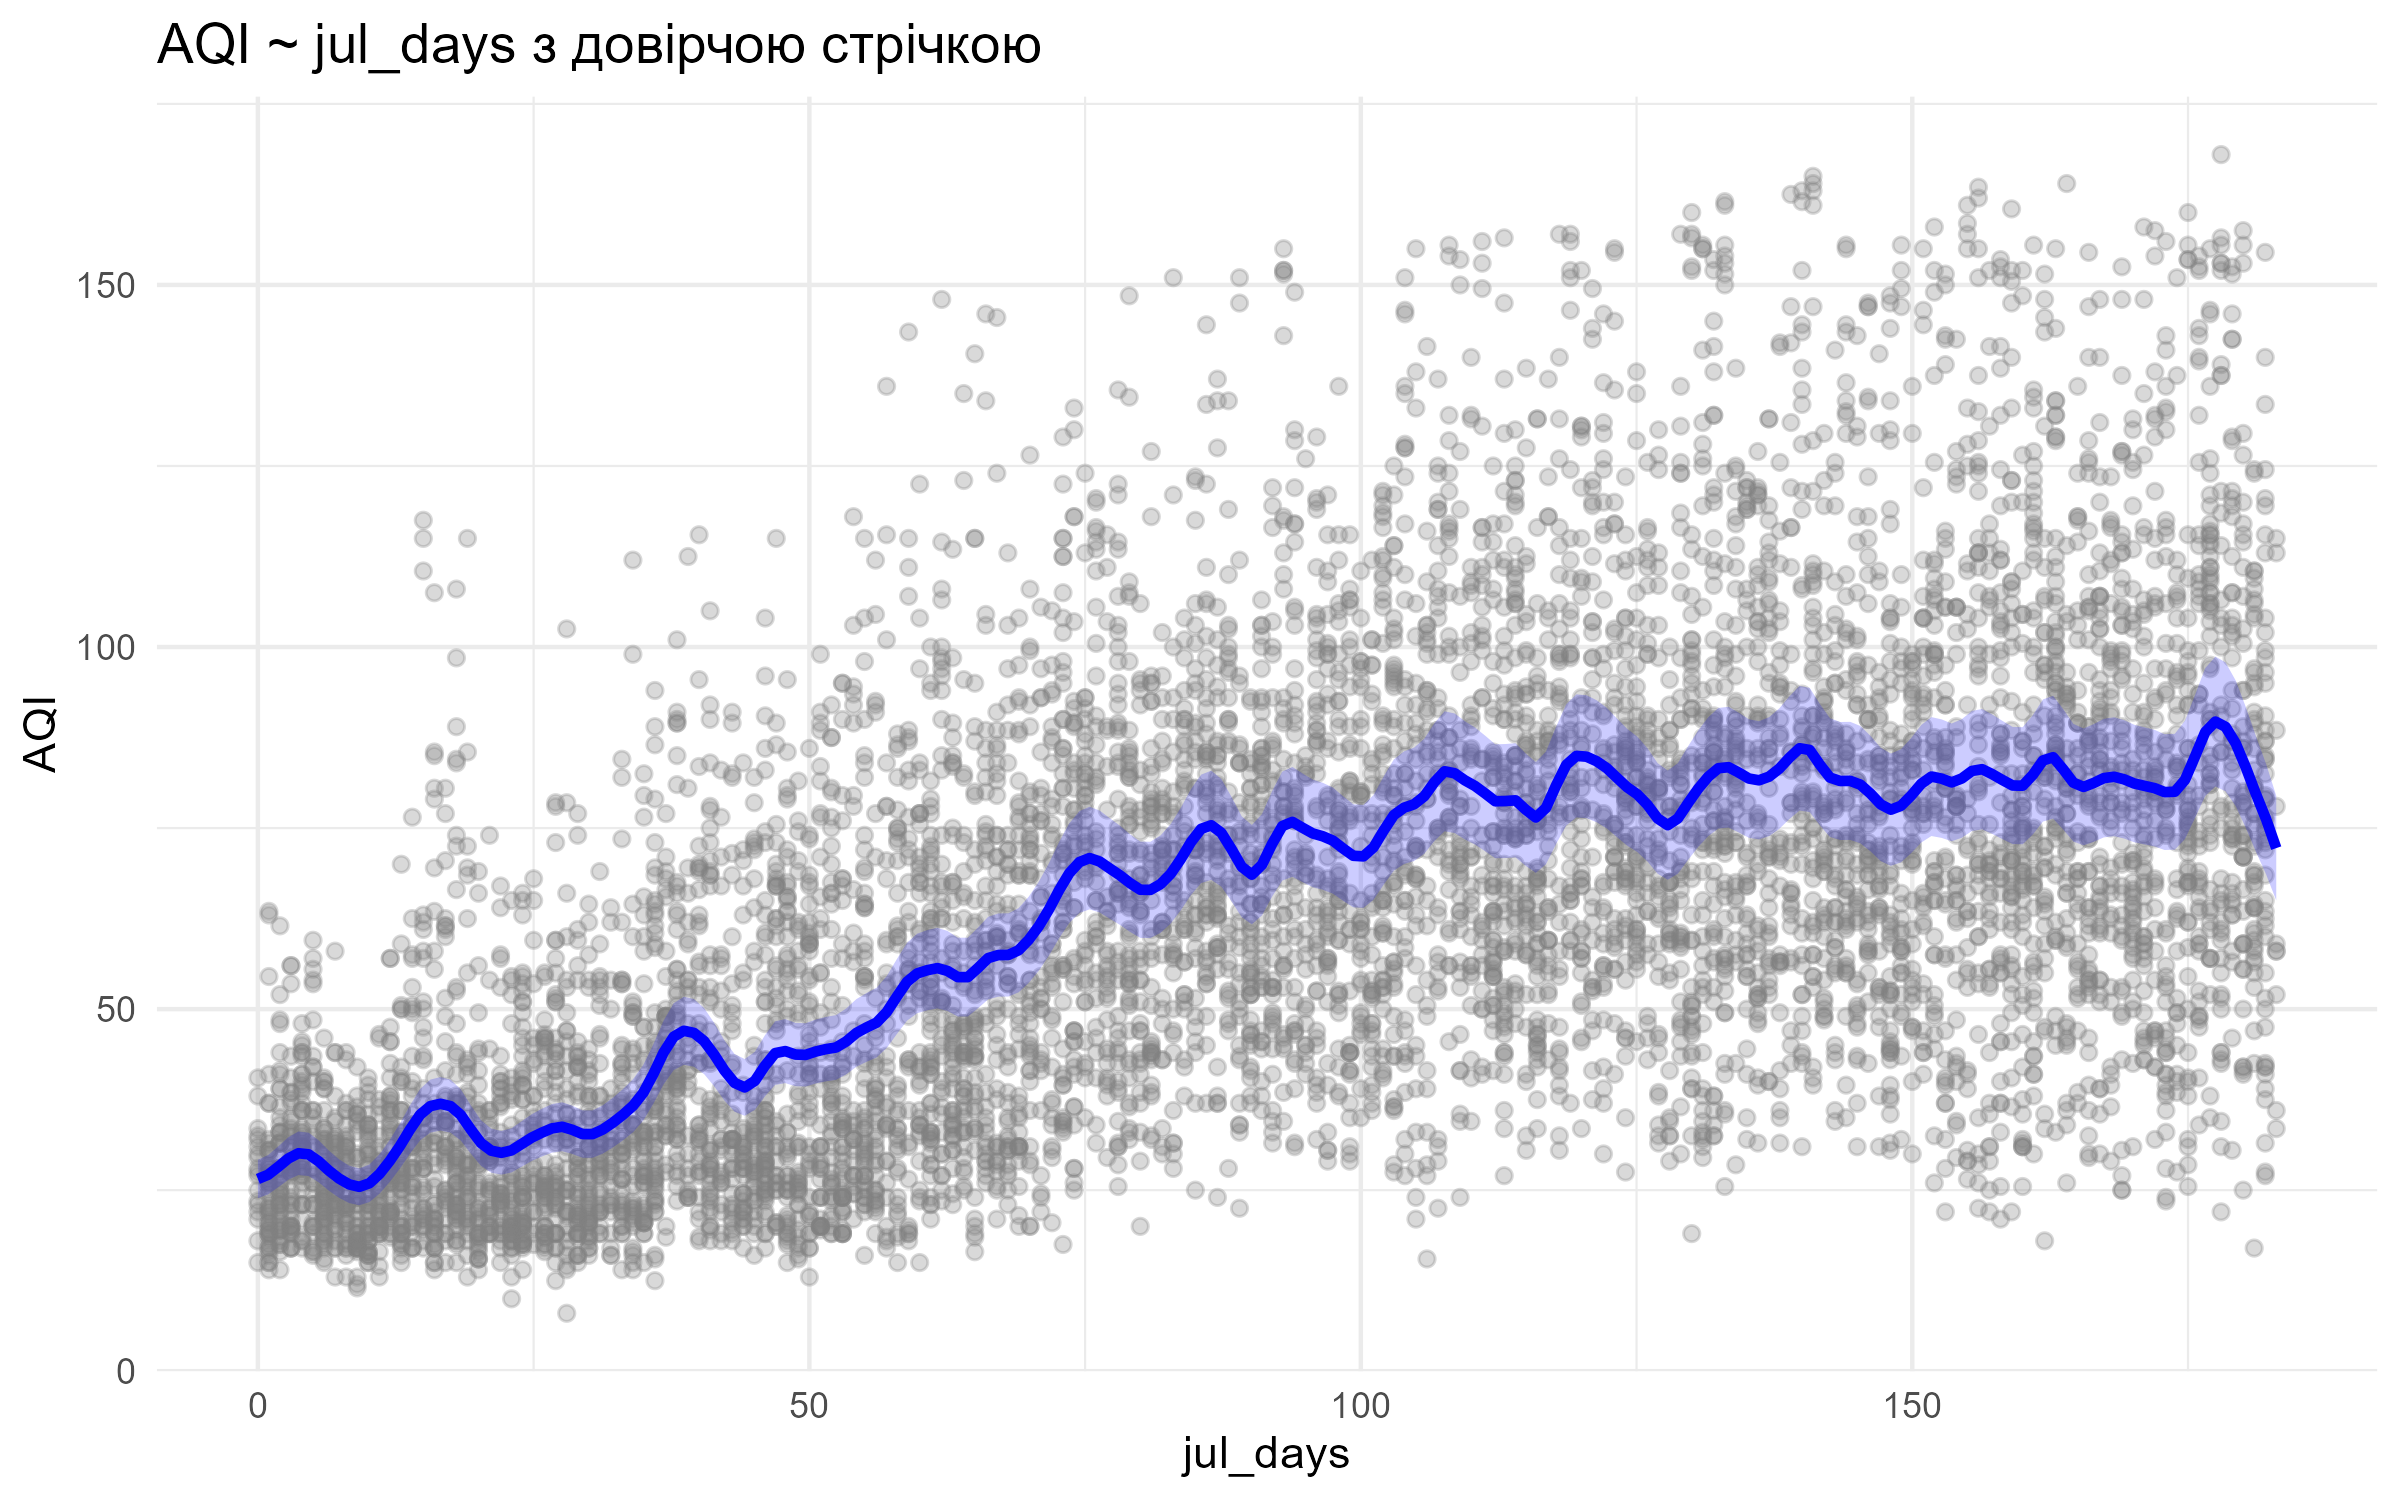
\includegraphics[height=2.8in]{plots/lab4/kernal/model1_fit_ribbon.png}
  \end{center}
 
  %\begin{itemize}
  %  \item \textbf{Локальна поліноміальна регресія (Local Polynomial Regression):}
  %  Узагальнення оцінки Надарая-Вотсона. Замість локального усереднення $Y_i$, вона апроксимує функцію регресії $m(x)$ локальним поліномом степеня $p$.
  %  Для локально-лінійної регресії ($p=1$), оцінка $\hat{\beta}_0$ в точці $x$ є оцінкою $m(x)$:
  %  $$ (\hat{\beta}_0, \hat{\beta}_1) = \arg\min_{\beta_0, \beta_1} \sum_{i=1}^{n} \left(Y_i - \beta_0 - \beta_1(X_i - x)\right)^2 K_h(X_i - x) $$
  %  Тоді $\hat{m}_h(x) = \hat{\beta}_0$.
  %  Локальні поліноми вищих порядків можуть краще адаптуватися до кривизни функції та зменшувати зміщення на границях.
  %\end{itemize}
\end{frame}

\begin{frame}
  \section{Частково-лінійна модель}

  \frametitle{Зміст}
  \tableofcontents[currentsection]
\end{frame}

\begin{frame}
  \frametitle{Розподіл регресорів}

\end{frame}

\begin{frame}
  \frametitle{Оцінка регресорів}

   \begin{center}
    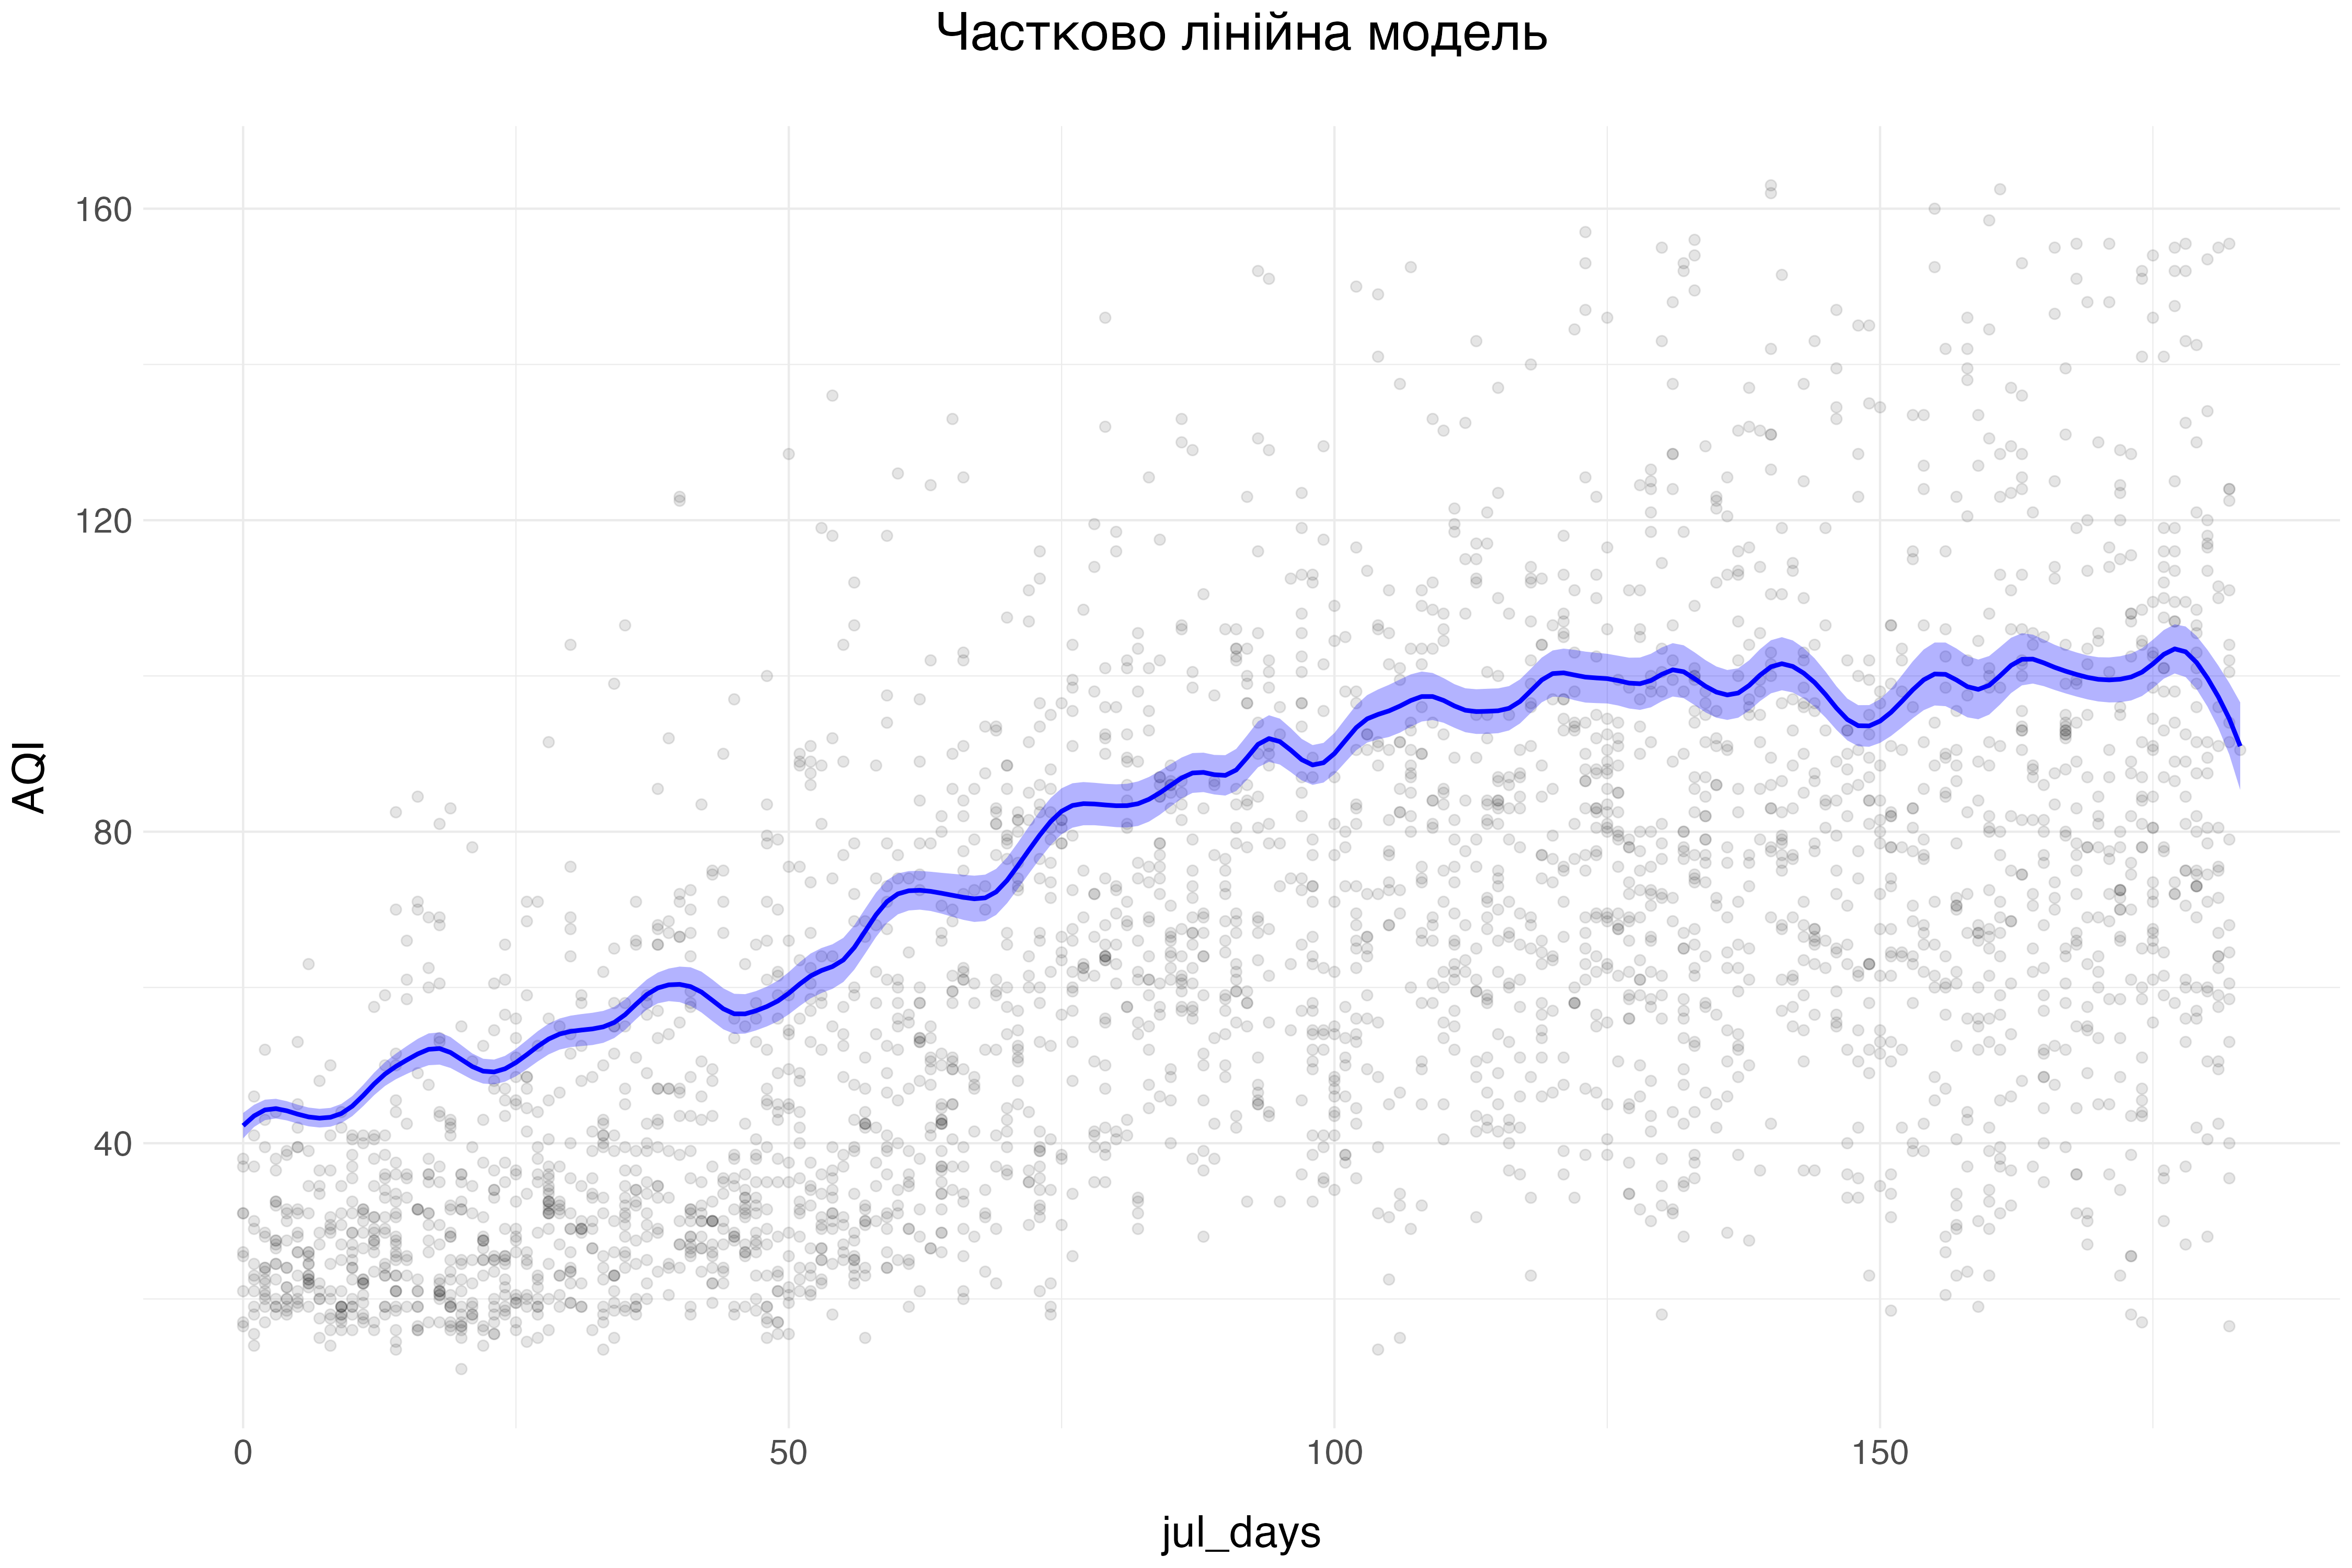
\includegraphics[height=2.8in]{plots/lab4/nppl.png}
  \end{center}
\end{frame}


\begin{frame}
  \section{Аналіз головних компонент}

  \frametitle{Зміст}
  \tableofcontents[currentsection]
\end{frame}

\begin{frame}
\frametitle{Аналіз головних компонент(Projection-1)}
  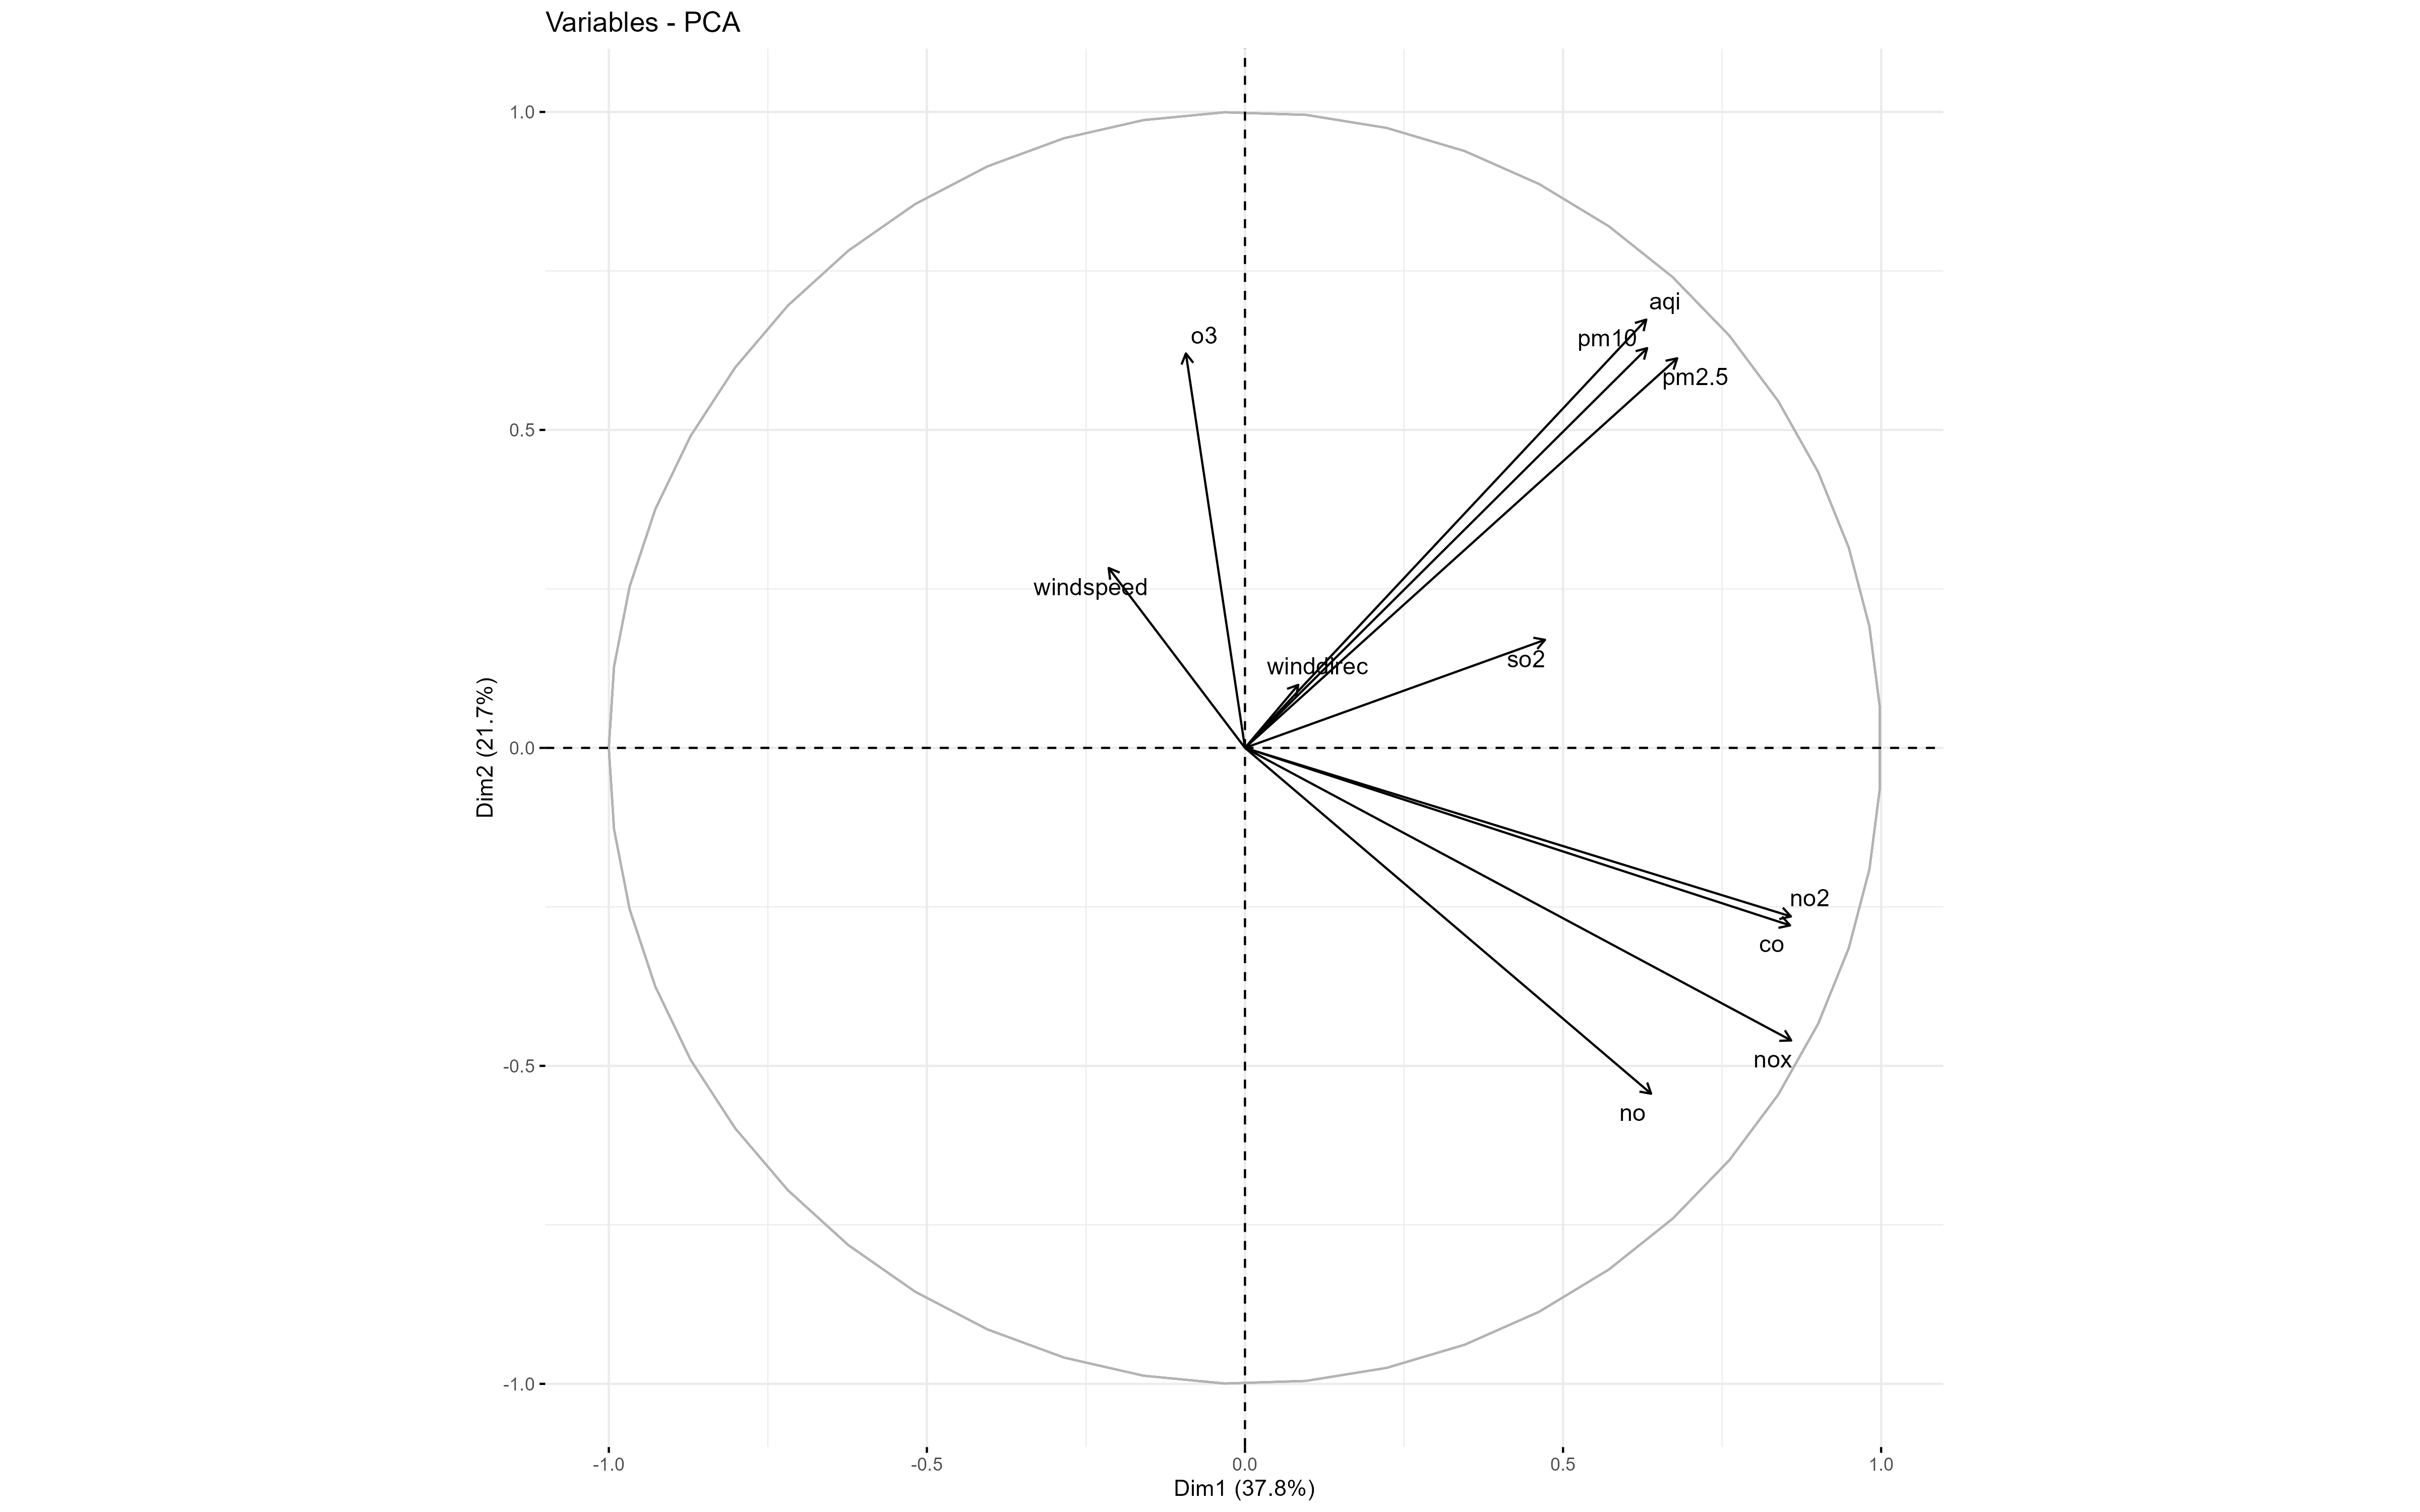
\includegraphics[height=2.8in]{plots/lab4/pca/projection-1-2.png}
\end{frame}

\begin{frame}
\frametitle{Аналіз головних компонент(Projection-2)}
  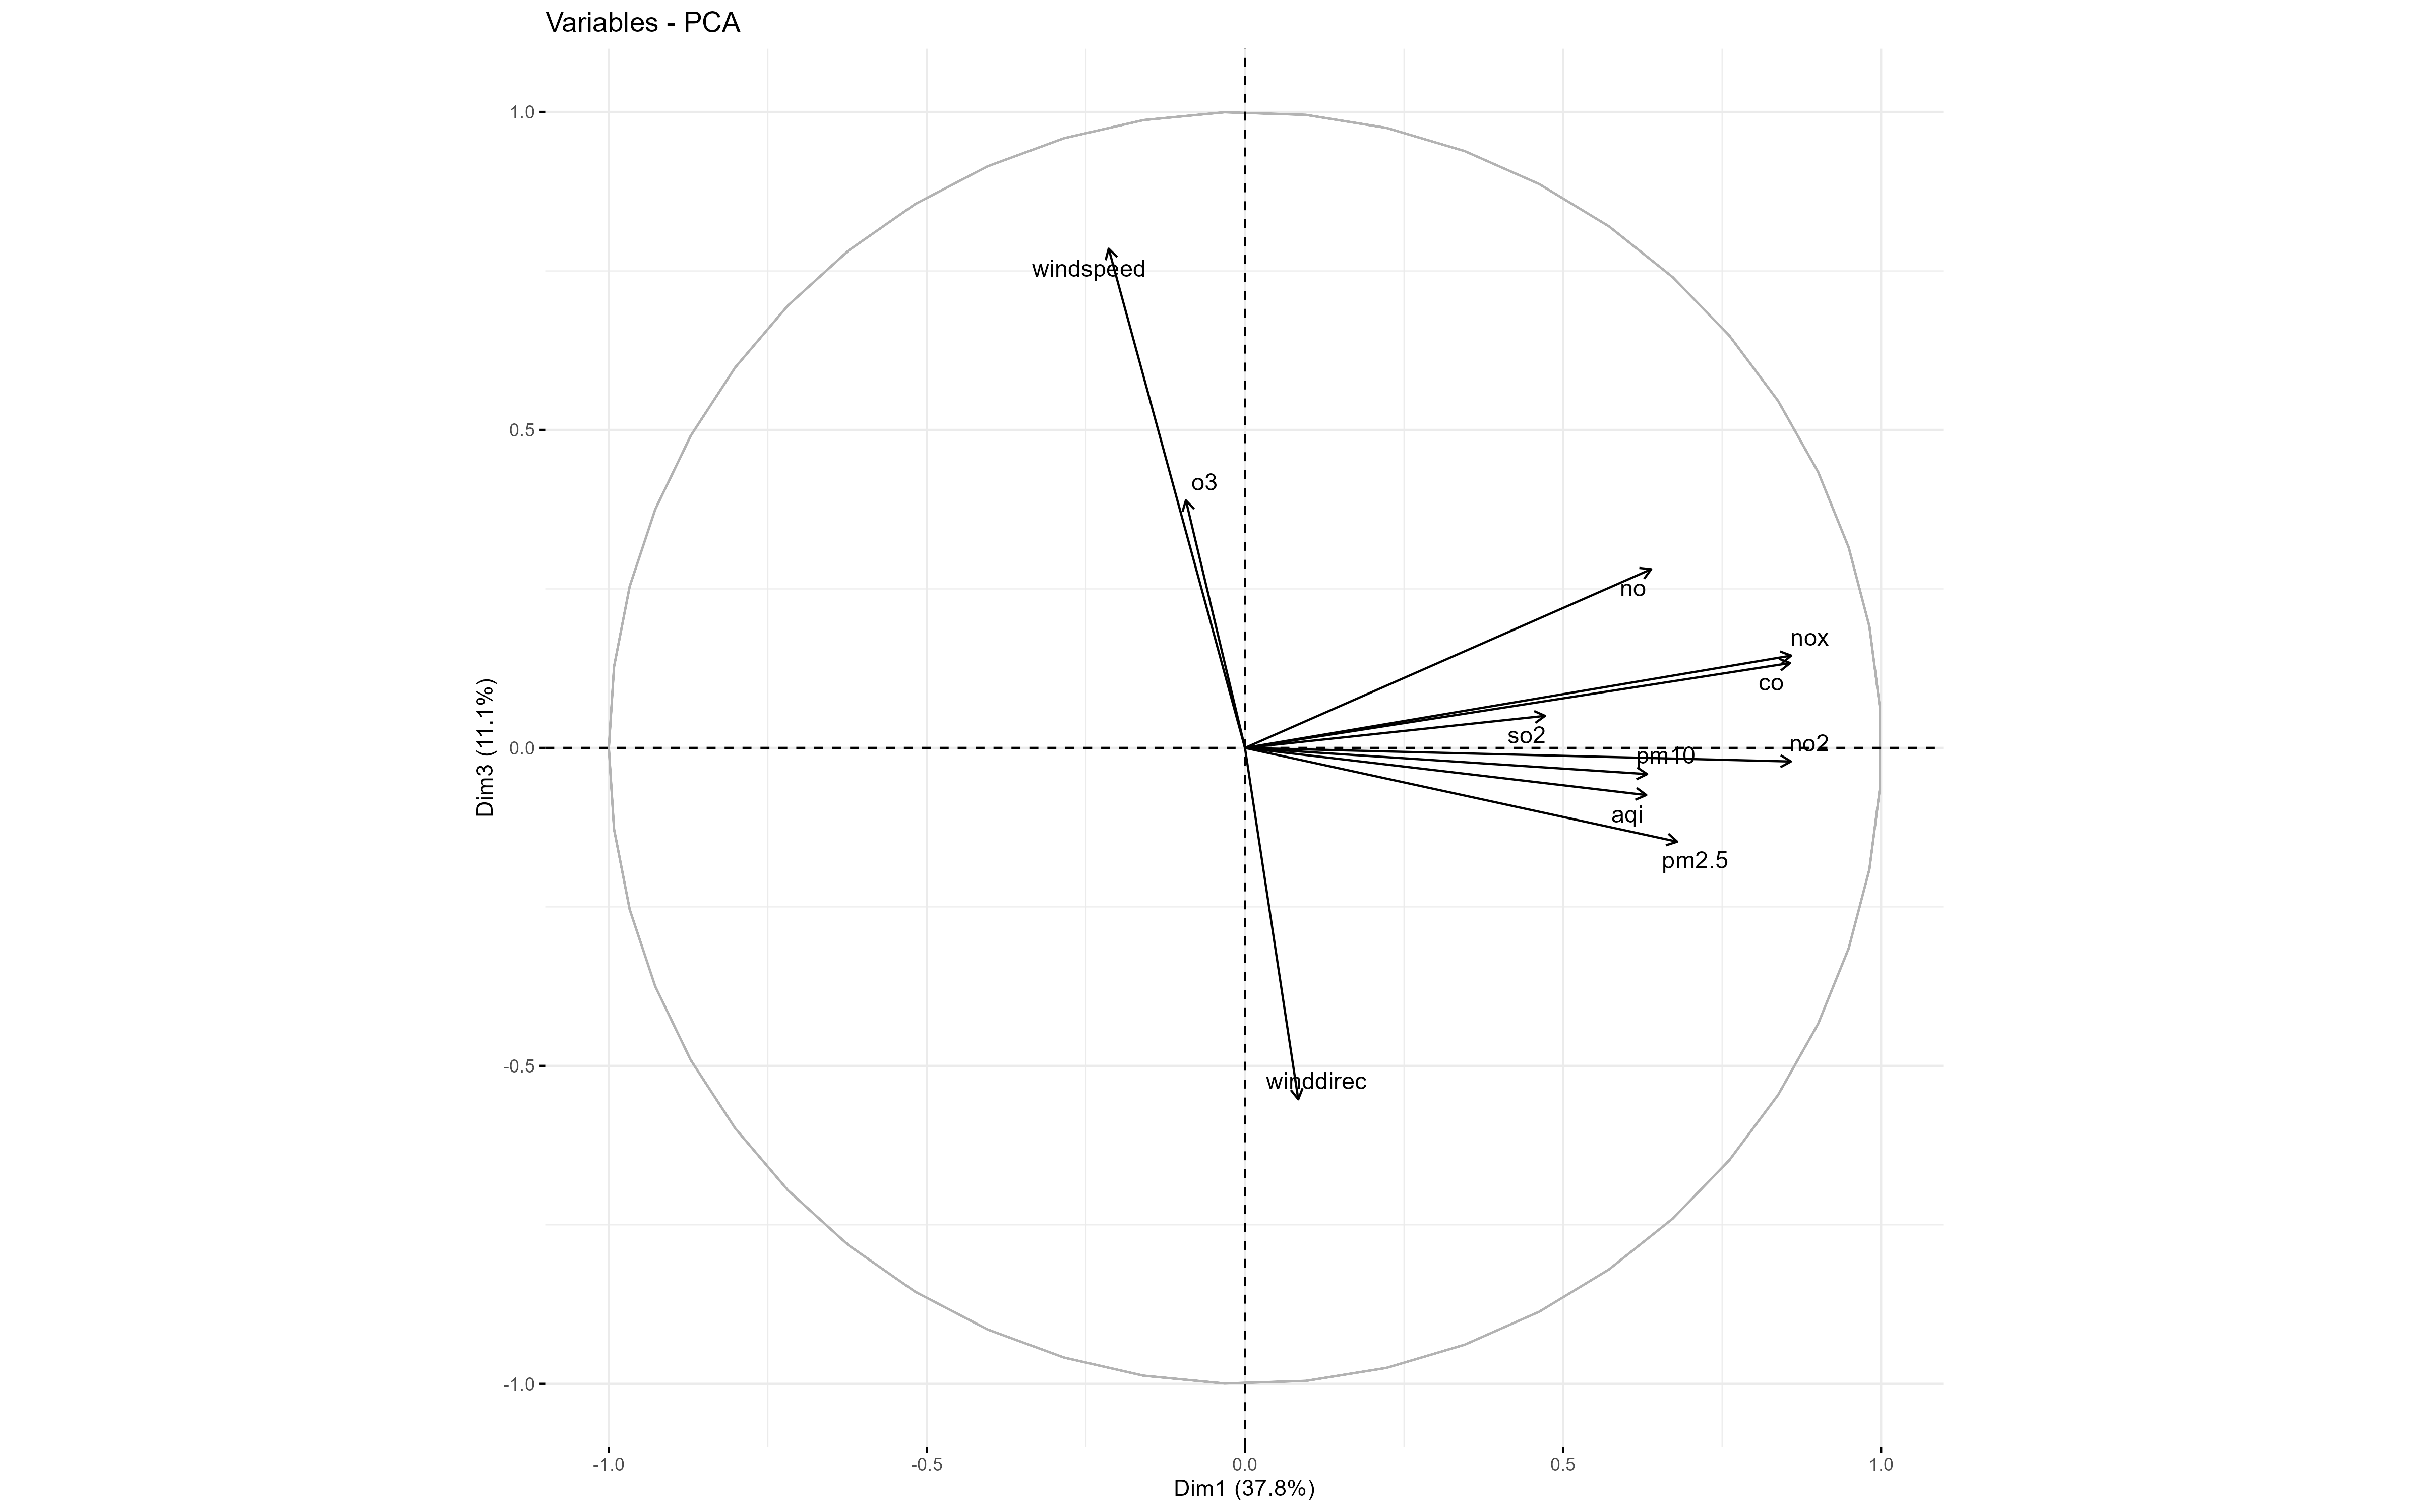
\includegraphics[height=2.8in]{plots/lab4/pca/projection-1-3.png}
\end{frame}

\begin{frame}
\frametitle{Аналіз головних компонент(Biplot)}
  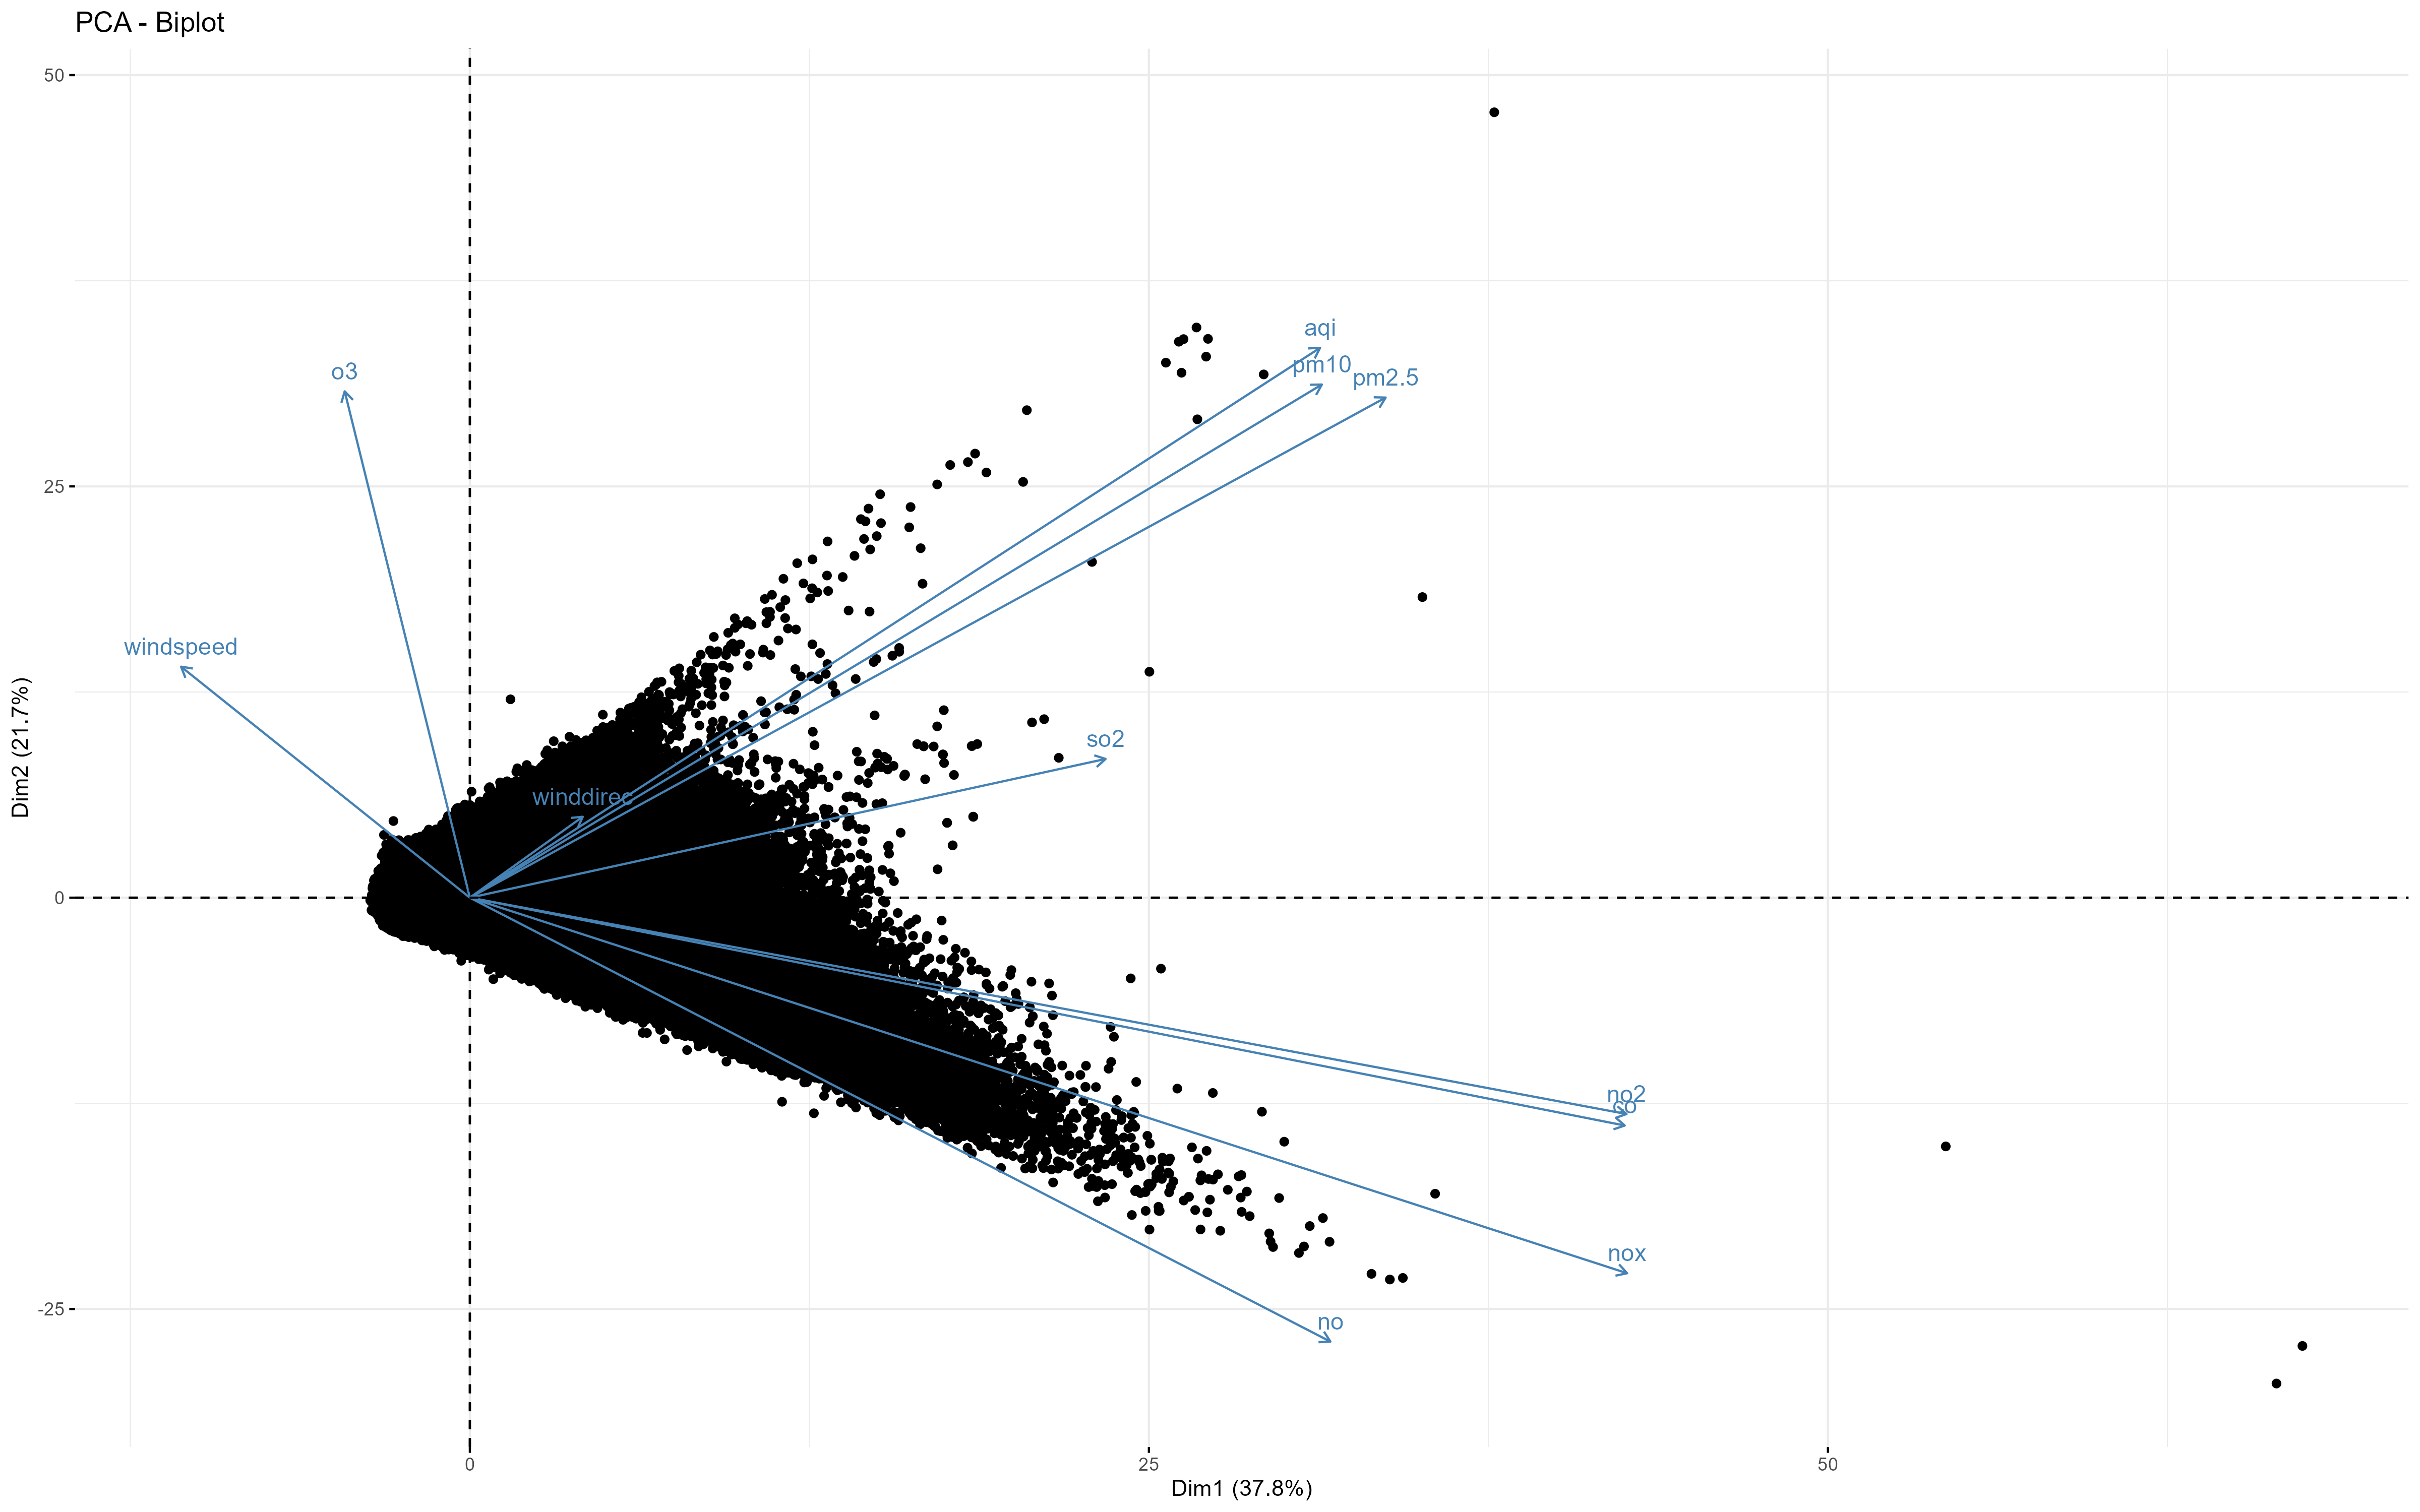
\includegraphics[height=2.8in]{plots/lab4/pca/biplot.png}
\end{frame}

\begin{frame}
\frametitle{Аналіз головних компонент(Scree plot)}
  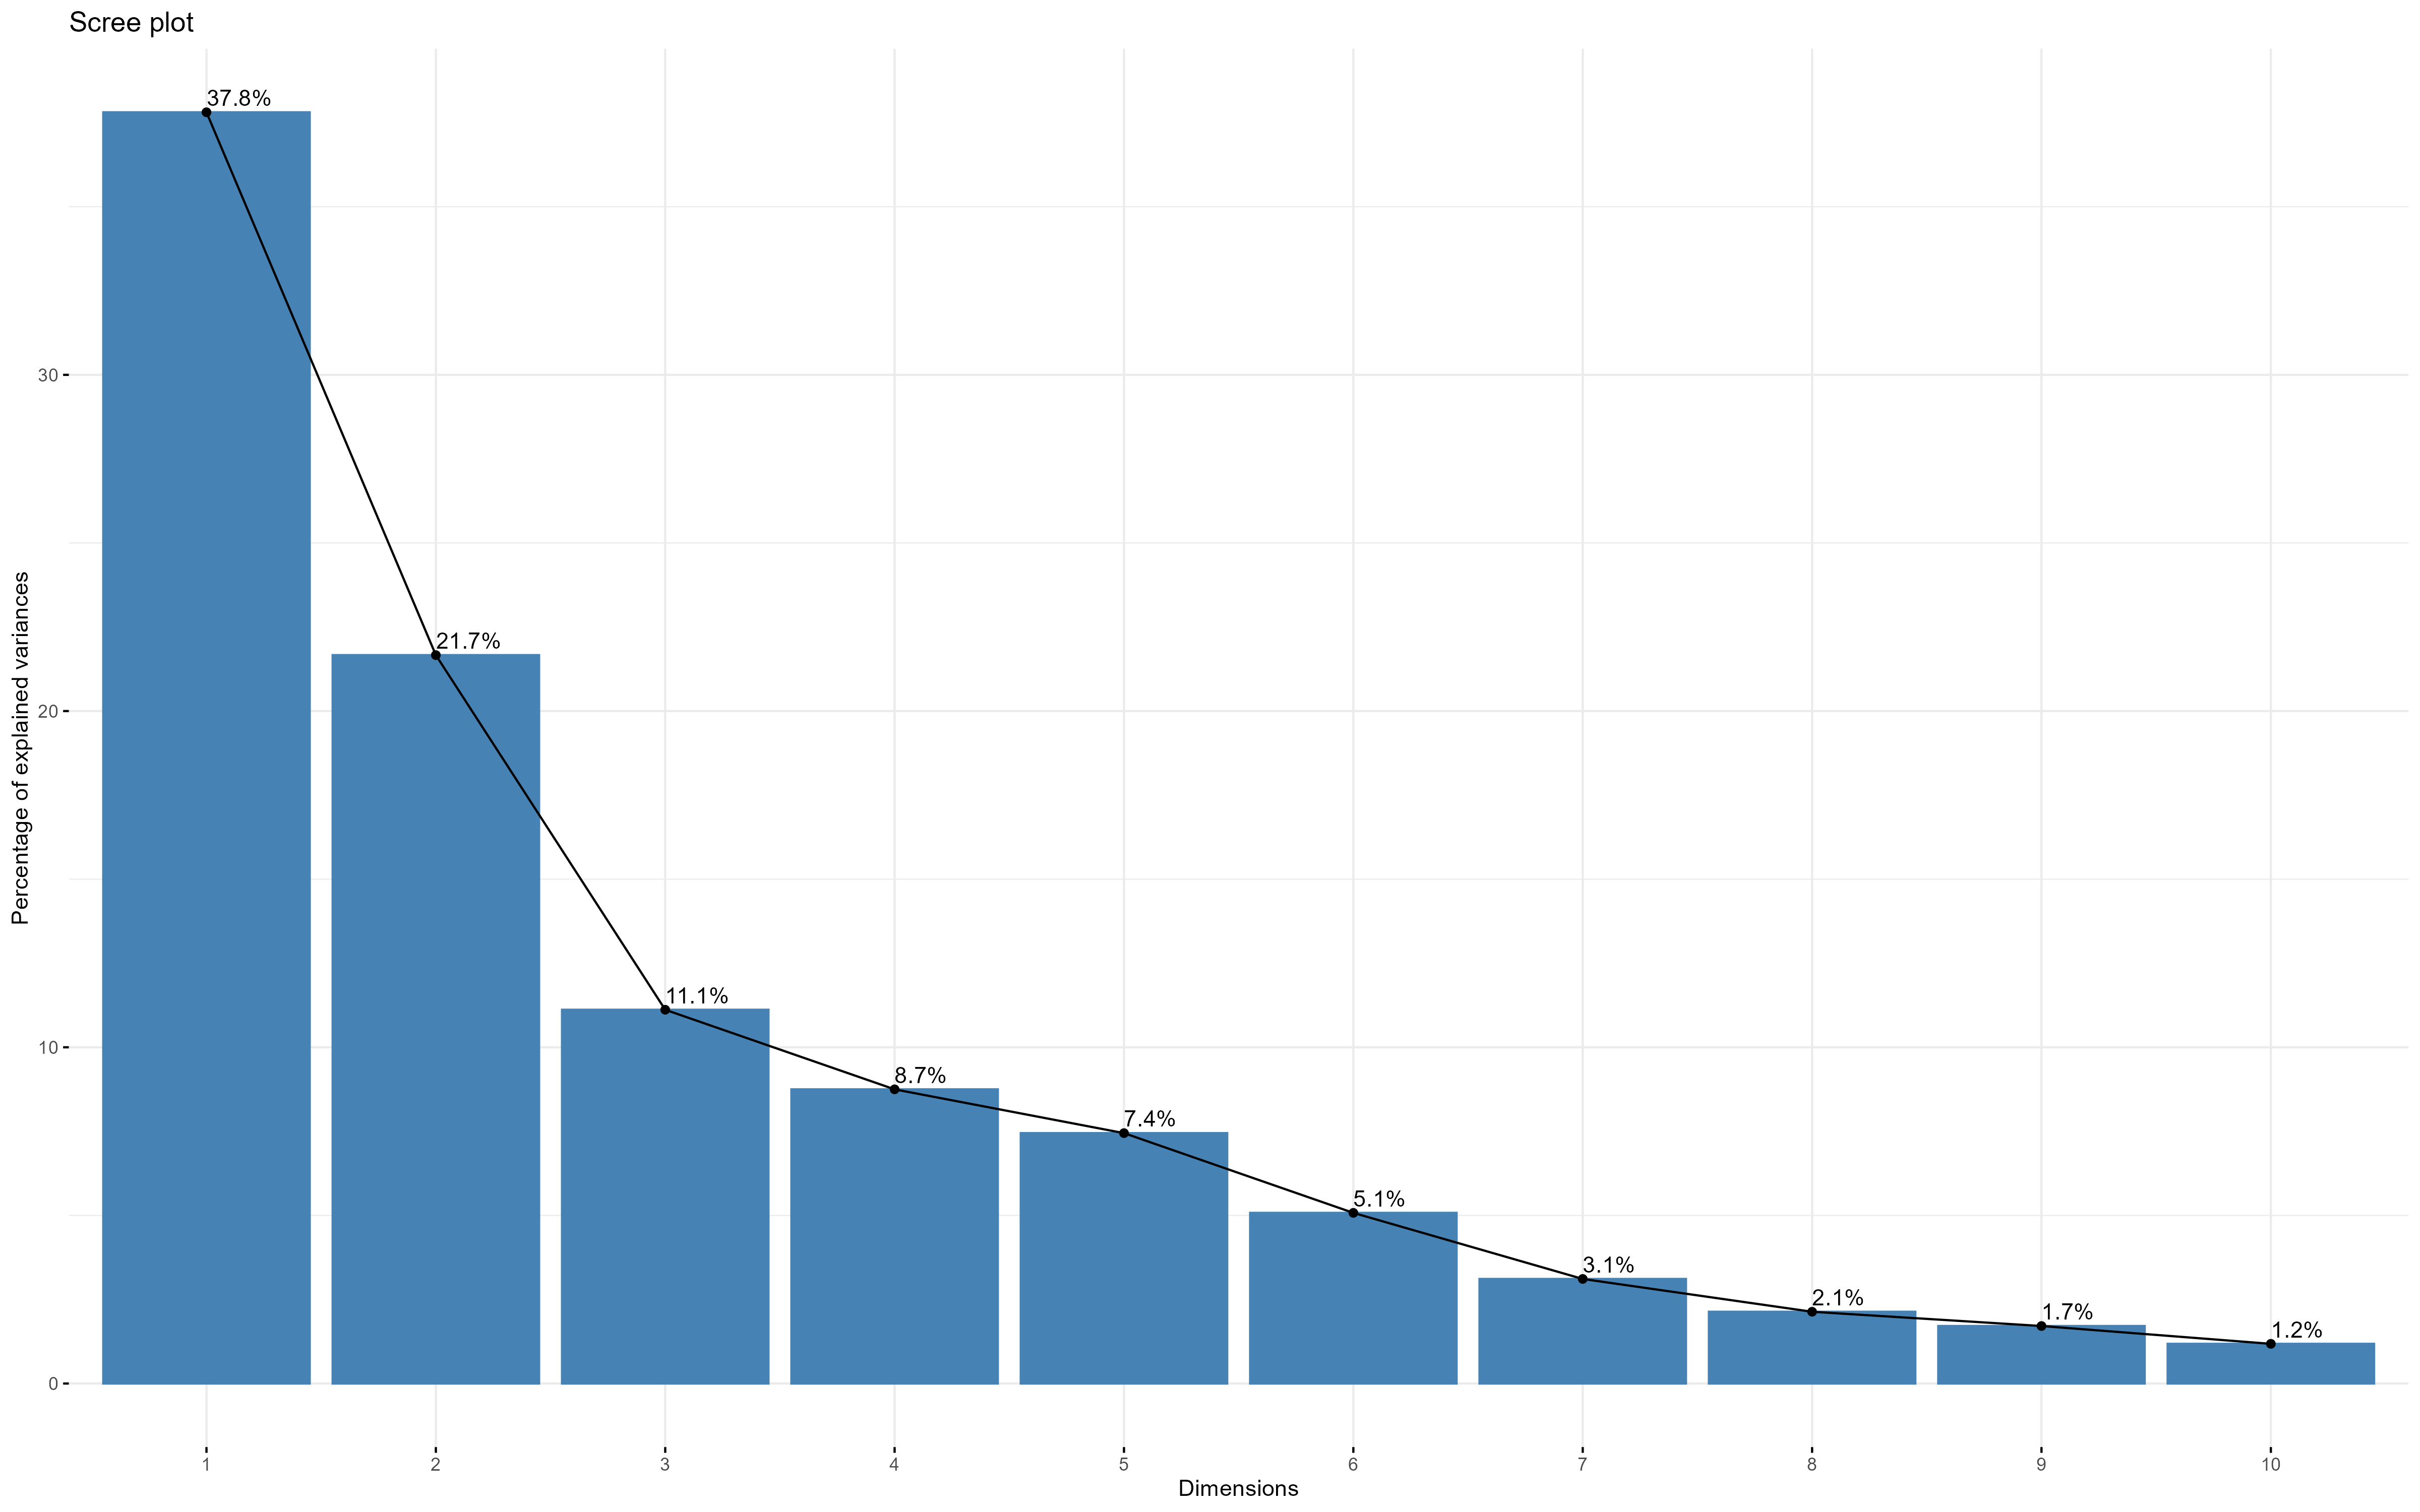
\includegraphics[height=2.8in]{plots/lab4/pca/scree.png}
\end{frame}

\begin{frame}
  \section{Порівняня результатів}

  \frametitle{Зміст}
  \tableofcontents[currentsection]
\end{frame}

\begin{frame}
  \frametitle{Порівняння ЛР3 (параметрична) та ЛР4 (непараметрична)}
  
\end{frame}

\begin{frame}
  \section{Висновок}

  \frametitle{Зміст}
  \tableofcontents[currentsection]
\end{frame}

\begin{frame}
  \frametitle{Висновок}
  % Підсумувати основні результати непараметричного аналізу.
  % - Які нелінійні залежності були виявлені та для яких змінних?
  % - Як непараметричні моделі доповнили/змінили розуміння, отримане з параметричних моделей (ЛР3)?
  % - Чи вдалося за допомогою PLM отримати збалансовану модель з інтерпретованими лінійними ефектами та гнучкою нелінійною компонентою?
  % - Відповідь на головне питання дослідження: Як реформа покращення якості повітря вплинула на якість повітря, враховуючи нелінійності?
  % - Обмеження дослідження та можливі напрямки для подальшої роботи.

  \begin{itemize}
    \item Непараметричний аналіз дозволив дослідити гнучкі форми залежностей AQI від ключових факторів, таких як \texttt{reform\_days} та \texttt{july\_days}, без апріорних припущень про їх функціональну форму.
    \item Частково-лінійна модель дозволила поєднати інтерпретованість лінійних ефектів для контрольних змінних з гнучкою оцінкою нелінійного впливу \texttt{some}.
  \end{itemize}

\end{frame}


\end{document}